
\documentclass[preprint]{sigplanconf}

% The following \documentclass options may be useful:

% preprint      Remove this option only once the paper is in final form.
% 10pt          To set in 10-point type instead of 9-point.
% 11pt          To set in 11-point type instead of 9-point.
% authoryear    To obtain author/year citation style instead of numeric.

\usepackage{amsmath}
\usepackage{amssymb}
\usepackage{amsthm}
\usepackage{amsfonts}
\usepackage{pifont}
\usepackage{listings}
\usepackage{graphicx}
\usepackage{xspace}
\usepackage{pgf}
\usepackage[noend]{algpseudocode}
\usepackage{algorithm}
\usepackage{multicol}
\usepackage{appendix}
\usepackage{caption}
\DeclareCaptionType{copyrightbox}
\usepackage{subfig}
\usepackage{multirow}
\usepackage{tikz}
\usetikzlibrary{arrows, automata, shapes}

\newtheorem{theorem}{Theorem}
\newtheorem{lemma}[theorem]{Lemma}
\newtheorem{corollary}[theorem]{Corollary}
\newtheorem{conjecture}[theorem]{Conjecture}

\theoremstyle{definition}
\newtheorem{definition}[theorem]{Definition}

\newcommand{\xmark}{\ding{55}}
\newcommand{\todo}[1]{{\bf TODO:} #1}

\lstset{language=c++}



\begin{document}

%\special{papersize=8.5in,11in}
\setlength{\pdfpageheight}{\paperheight}
\setlength{\pdfpagewidth}{\paperwidth}

\conferenceinfo{POPL '14}{Month d--d, 20yy, City, ST, Country} 
\copyrightyear{2014} 

% Uncomment one of the following two, if you are not going for the 
% traditional copyright transfer agreement.

%\exclusivelicense                % ACM gets exclusive license to publish, 
                                  % you retain copyright

%\permissiontopublish             % ACM gets nonexclusive license to publish
                                  % (paid open-access papers, 
                                  % short abstracts)

\title{Synthesising Complex Termination Arguments}

\authorinfo{Cristina David\and Daniel Kroening\and Matt Lewis}
           {Oxford University}
           {firstname.lastname@cs.ox.ac.uk}

\maketitle

\begin{abstract}
Proving program termination is typically done by finding a well-founded \emph{ranking function}
for the program states.
Existing termination provers typically find ranking functions
using either linear algebra or templates.  As such they are often restricted to
finding linear ranking functions over mathematical integers.  This class
of ranking functions is not large enough to prove termination for all terminating
programs, and furthermore a termination argument for a program operating on mathematical integers
does not always lead to a termination argument for the same program operating on
fixed-width machine integers.

We present a reduction from program \emph{termination} to program \emph{synthesis}.
This reduction allows us to generate nonlinear, lexicographic ranking functions that
are correct for fixed-width machine arithmetic and floating-point arithmetic.
We use this reduction to build a semi-decision procedure for the termination
of fixed-width and floating-point arithmetic programs.
\end{abstract}

%\category{CR-number}{subcategory}{third-level}


\keywords
Termination, Program Synthesis, Lexicographic Ranking Functions, Bitvector Ranking Functions,
Floating Point Ranking Functions.

\section{Introduction}\label{sec:intro}

Proving program termination is typically done by finding a \emph{ranking function}
for the program states, i.e. a map from the program's state space to a well-ordered set.
%% As this definition of a ranking function is very general, research is often limited to some
%% convenient and tractable form of ranking functions, most frequently \emph{linear ranking functions} (see Section~\ref{sec:ranking.functions}). 
%% In doing so, an analysis ensures that such a ranking function will be found if one  exists, 
%% while failing to prove termination for terminating programs whose ranking functions fall short of the considered restriction. 
In doing so, the majority of the existing termination provers diverge 
in one important aspect from the execution of a program on a computer:
bit-vectors and floats are treated as mathematical integers and reals, respectively.
Figure~\ref{fig:handletable} presents a summary of existing termination analyses with indeed
most of them designed for integers and assuming a \emph{restrictive transition relation}, e.g. linear programs \cite{DBLP:conf/pldi/CookPR06,DBLP:conf/popl/Ben-AmramG13,DBLP:conf/vmcai/P04,DBLP:conf/atva/HeizmannHLP13,DBLP:conf/vmcai/BradleyMS05,DBLP:conf/cav/KroeningSTW10}. 
% \emph{linear ranking functions for linear programs over integers}.
These design decisions may give rise to 
{\em unsound} and {\em incomplete} analyses, as discussed next.
%which is rather surprising given that bit-vectors and floats are ubiquitous in computer systems. 

%\noindent {\bf Bit-vectors (machine-level integers) vs. mathematical integers.} 

Physical computers have bounded storage, which means they are unable to perform calculations on mathematical
integers.  For example, if $A$ is the Ackermann function and $G$ is Graham's number, a physical computer
capable of computing $A(G, G)$ would contain (much!) more matter than is believed to exist in the universe.
Fortunately, it is rare for a programmer to need such a large number and so modern computers do their arithmetic
over fixed-width binary words, otherwise known as bit-vectors.

%Bit-vector arithmetic is very similar to modular arithmetic.  For a computer using $k$-bit words, unsigned
%calulcations are just defined to 
The abstraction of bit-vectors to mathematical integers 
ignores the wrap-around behaviour caused by under/over-flows in bit-vector arithmetic, resulting in 
incomparable behaviours with respect to termination. 
%The loop in Figure~\ref{} terminates for integers, but does not terminate for bit-vectors. 
The loop in Figure~\ref{} always terminates for unbounded integers as the value of \texttt{x} does eventually become negative, 
whereas, with bit-vector arithmetic, \texttt{x} under-flows before becoming negative and goes back to being positive causing the loop to never terminate.
%% =======
%% most of the work concentrated on finding \emph{linear ranking functions for linear programs over integers}.
%% Next, we will consider in more detail the assumptions made by such techniques and their implications.\\

%% \noindent {\bf Bit-vectors (machine-level integers) vs. mathematical integers.}
%% Physical computers have bounded storage, which means they are unable to perform calculations on mathematical
%% integers.  For example, if $A$ is the Ackermann function and $G$ is Graham's number, a physical computer
%% capable of computing $A(G, G)$ would contain (much!) more matter than is believed to exist in the universe.
%% Fortunately, it is rare for a programmer to need such a large number and so modern computers do their arithmetic
%% over fixed-width binary words, otherwise known as bit-vectors.

%% Bit-vector arithmetic is very similar to modular arithmetic.  For a computer using $k$-bit words, unsigned
%% calulcations are just defined to 

%% The abstraction of bit-vectors to mathematical integers 
%% ignores the wrap-around behaviour caused by under/over-flows in bit-vector arithmetic, resulting in %, it gives rise to 
%% %{\em unsound} and {\em incomplete} analyses, which is rather surprising given that bit-vectors are ubiquitous in computer systems. 
%% incomparable behaviours with respect to termination:
%% %The differences between the semantics of unbounded mathematical integers and that of machine integers result in 
%% \begin{itemize}
%% \item Programs that terminate for integers may \emph{not} terminate for bit-vectors. For illustration, consider the following loop:
%% \begin{lstlisting}[language=C]
%% while (x > 0) x -= 2;
%% \end{lstlisting}
%% The loop always terminates for unbounded integers as the value of \texttt{x} does eventually become negative, 
%% >>>>>>> 7b690c08a70e4161a432600e9456d922106badaf
According to the C11 standard for the C programming language, a signed under- or over-flow yields undefined behaviour.
However, compilers generally treat signed under- and over-flows using the
wrap-around behaviour (see Section~\ref{sec:machine.arith}). %This means that a termination analysis for integers would return an unsound result for this situation.
As a second example, the loop in Figure~\ref{} is  terminating for bit-vectors since \texttt{x}
will eventually over-flow and become negative. Conversely, the same program is non-terminating using integer
arithmetic since the loop condition stays always true for any initial \texttt{x} at least 1.

%Similarly, programs that terminate for bit-vectors may \emph{not} terminate for integers. One such situation is illustrated next:  

\begin{lstlisting}[language=C]
while (x > 0) x -= 2;
\end{lstlisting}

\begin{lstlisting}[language=C]
 while(x > 0) x++;
 \end{lstlisting}

%\noindent {\bf Floats vs. reals.} 
A scenario similar to the one for bit-vectors happens if floats were to be abstracted to unbounded reals by termination provers \cite{}. 
Consequently, these provers ignore potential rounding errors, under- and over-flows, which are precisely what makes  reasoning about floating point inherently difficult.
This approximation may lead to erroneous diagnosis of a program's terminating behaviour as illustrated by the loops in Figure~\ref{} and Figure~\ref{}.
While the former does not terminate for reals, but does for floats, the latter 
terminates for reals, but does not for floats.

\begin{lstlisting}
while (x > 0.0) x *= 0.5;
\end{lstlisting}

\begin{lstlisting}
while (x > 0.0) x -= 1.0;
\end{lstlisting}
\todo{explain the reasons for non-termination with figures.}\\


%% \noindent {\bf Linear programs and linear ranking functions.} As visible in Figure~\ref{fig:handletable}, 
%% most termination techniques assume \emph{restrictive transition relations}, e.g. linear programs,  and are only able to compute
%% \emph{linear ranking functions} \cite{}. To better understand this restriction, we computed the probability of a random terminating program having a linear ranking
%% function (see Section ?). This probability proved to be very low, indicating that the linearity assumption for the ranking functions is indeed prohibitive.


If we survey the area of program termination chronologically, we observe an initial domination of  monolithic approaches based on a single measure shown to decrease
over all program paths %(syntactic characterisation of loops) 
\cite{DBLP:conf/vmcai/P04,DBLP:conf/cav/BradleyMS05}, followed by 
more recent techniques moving towards termination arguments based on Ramsey's theorem \cite{DBLP:conf/lpe/CodishG03,DBLP:conf/lics/PodelskiR04,DBLP:conf/pldi/CookPR06}.
The latter approach aims to find a set of local termination conditions that decrease as execution follows through the loop. %(semantic characterisation of loops).
The main justification for this paradigm shift lies in the simplicity of the local termination measures when compared to the global ones, e.g.
there are cases in which proofs based on local measures involve applying linear functions while corresponding global
measures involve nonlinear functions or lexicographic orders.


The downside of a Ramsey-based approach is the fact that a valid termination argument must hold for the \emph{transitive closure}
of the program's transitions, rather than only for individual transitions. 
As such, there is experimental evidence that most of the time is spent in reachability analysis \cite{DBLP:conf/pldi/CookPR06}, 
requiring the support of powerful safety checkers.
Basically, these approaches opt for simpler termination arguments in the detriment of complex validity checking.


As Ramsey-based approaches are limited by the state of the art in safety checking, 
recent research shifts back to more complex termination arguments that are easier to check \cite{DBLP:conf/tacas/CookSZ13,DBLP:conf/cav/KroeningSTW10}.
%In \cite{DBLP:conf/tacas/CookSZ13}, Cook et al present an iterative termination proving procedure that searches for 
%lexicographic termination arguments, whereas Kroening et al. strengthen the termination argument such that it becomes a transitive relation \cite{DBLP:conf/cav/KroeningSTW10}.
%
%
Following the same trend, %of switching the complexity in termination checking back to the termination arguments, 
we investigate its very extreme: \emph{unrestricted} termination arguments. 
This means that our ranking functions may involve non-linearity and lexicographic orders (we do not commit to any such form, i.e. we do not use templates).
That is, we propose a general framework that does not assume the existence of linear ranking functions and can uniformly compute
\emph{lexicographic/non-lexicographic} \emph{linear/non-linear} 
ranking functions supported by inductive \emph{linear/non-linear} invariants for loops with 
\emph{linear/non-linear} guards and transitions over bit-vectors and floats.
Our technique is {\emph complete} and can handle programs with non-linear operations, e.g. logical and.
In our design, the termination problem becomes as hard as finding ranking functions, rather than as hard as
checking the validity of a termination argument. 

 
Given the level of generality that we aim for, we phrase the termination problem as a second order satisfaction problem (indeed, a program synthesis problem) (Section~\ref{}).
While investigating the search space and the distribution of solutions (Section~\ref{}), we identify factors influencing our method's performance and
find that our technique %is semantic in nature and 
does not dependent on the size of the analysed program or its number of variables, but on the Kolmogorov
 complexity of the computed ranking functions. We show that the probability of
a ranking function to have a low Kolmogorov complexity is higher than the probability to be linear (see Section~?).
Moreover, we find that our technique does actually gain from the generality of the termination argument. 
After investigating its theoretical bounds, we experimentally show that our technique performs well in practice. 


\begin{figure*}
\centering
 \begin{tabular}{|ll||c|c|c|c|c|c|c|c|}
 \hline
  & & \multicolumn{8}{c|}{Program} \\
  & & \multicolumn{2}{c|}{Integers} & \multicolumn{2}{c|}{Reals} & \multicolumn{2}{c|}{Bit-vectors} & \multicolumn{2}{c|}{Floats} \\
  & & L & NL & L & NL & L & NL & L & NL \\
  \hline
  \hline
  \multirow{4}{*}{Ranking} & Linear lexicographic &  \cite{DBLP:conf/cav/BradleyMS05,DBLP:conf/tacas/CookSZ13,DBLP:conf/vmcai/P04} && & &\checkmark&\checkmark&\checkmark&\checkmark\\
   & Linear non-lexicographic & \cite{DBLP:conf/pldi/CookPR06,DBLP:conf/cav/LeeWY12,DBLP:conf/popl/Ben-AmramG13,DBLP:conf/vmcai/P04,DBLP:conf/atva/HeizmannHLP13,DBLP:conf/vmcai/BradleyMS05,DBLP:conf/cav/KroeningSTW10} & \cite{DBLP:conf/vmcai/BradleyMS05} & && \checkmark~ \cite{DBLP:conf/tacas/CookKRW10} &\checkmark~ \cite{DBLP:conf/tacas/CookKRW10}&\checkmark&\checkmark\\
   & Non-linear lexicographic &  &  & &&\checkmark&\checkmark&\checkmark&\checkmark\\
   & Non-linear non-lexicographic & \cite{DBLP:conf/vmcai/BradleyMS05} &  \cite{DBLP:conf/vmcai/BradleyMS05} & &&\checkmark&\checkmark&\checkmark&\checkmark\\
   \hline
 \end{tabular}

 \caption{Legend: \checkmark = we can handle\label{fig:handletable}}
\end{figure*}


%We empirically observe that most programs have
%ranking functions with low Kolmogorov complexity (see Section ?). 

%Church was BIG into program synthesis~\cite{church-synth}, so you know it's good stuff.
%Something, something, Curry-Howard Isomorphism, something, something, programs-as-proofs.

 The main contributions of our work can be summarised as follows:
\begin{itemize}
\item We designed a technique for computing ranking functions that correctly accounts for the wrap-around behavior caused by under- and overflows in bit-vector and floating point arithmetic. To the best of our knowledge, this is the first approach able to compute ranking functions for programs handling floats. Our technique is not restricted to finding linear ranking functions, but can also compute (lexicographic) non-linear  ones. We justified the need for such a non restrictive procedure by computing the probability ... .
\item  We rephrased the termination problem as a second-order satisfaction problem and made 
use of results in genetic programming to efficiently solve it. We have also investigated the effects of genetic operators on the search space for ranking functions and computed theoretical 
bounds on the convergence time ...
\item We present a formulation that allows us to prove termination without an expensive reachability check (as we don't use Ramsey-based termination arguments).  In particular,
we only need a bounded model checker that performs a single unwinding of a loop.
%% \item Our technique is able to uniformly handle conditionally-terminating loops, as well as programs with
%% multiple loops.
\item We implemented our technique and tried it on a selection of programs handling both bit-vectors and floats.
\end{itemize}

%. only non-strict inequalities can be transformed using Farkas’ Lemma
%--Our approach to termination analysis has two distinct features over previous works
%-- a lexicographic ranking function imposes a lexicographic ordering on among the ranking function components.

% The main advantage of our approach is its unitary nature. We do not require any initial assumption regarding the form of the termination  
% argument, as this does not influence our search process. We identify the factors influencing the performance of our design and 
% show that these factors are independent on the linearity of the ranking function or the number of lexicographic components...


%semantic approach

%given that the search space size is constant, the probability of finding a solution 
%increases when considering all the possible solutions. There is no point in restricting the form of the solution..
%to read: constraint-based.., integers vs rationals.

%This paper is organised as follows:

\section{Related Work}
%\subsection{Termination analysis}
Automated program termination is a research topic that has received a fair amount of attention from the software verification community.
In order to compare our technique to the rest of the area, 
Figure~\ref{fig:handletable} summarises the related works with respect to the restrictions they impose on the transition relations as well as the form of the computed ranking functions. 


Somehow expected, most of the techniques are specialised in the synthesis of linear ranking functions for linear programs over integers (or rationals) \cite{DBLP:conf/pldi/CookPR06,DBLP:conf/cav/LeeWY12,DBLP:conf/popl/Ben-AmramG13,DBLP:conf/vmcai/P04,DBLP:conf/atva/HeizmannHLP13,DBLP:conf/cav/BradleyMS05,DBLP:conf/tacas/CookSZ13}. 
Among them, 
Lee et al. make use of transition predicate abstraction, algorithmic learning, and decision procedures to compute transition
invariants as proofs for the termination of linear programs \cite{DBLP:conf/cav/LeeWY12}.
Leike and Heizmann present a new method for the constraint-based synthesis
of termination arguments for linear loop programs based on
linear ranking templates \cite{DBLP:conf/tacas/LeikeH14}.
Linear ranking functions supported by inductive linear invariants for loops with linear guards and transitions: \cite{DBLP:conf/cav/BradleyMS05}. 
Learning: \cite{DBLP:journals/corr/HeizmannHP14}


%A program is lasso-shaped if it is composed by a stem followed by a single loop without branching, i.e. there is only one path. 
%Consequently, the termination argument can be very simple. There are numerous techniques specialised in
%proving termination of lasso-shaped programs efficiently \cite{DBLP:conf/popl/Ben-AmramG13,DBLP:conf/cav/BradleyMS05,DBLP:conf/atva/HeizmannHLP13,DBLP:conf/vmcai/P04}. 

While the synthesis of termination arguments for linear programs over integers is indeed well-covered in the literature, 
there is very limited work for programs over machine integers.
Cook et al. present a method based on a reduction to Presburger
arithmetic, and a template-matching approach for predefined classes of
ranking functions based on reduction to SAT- and QBF-solving \cite{DBLP:conf/tacas/CookKRW10}.
Similarly, the only work we are aware of that can compute non-linear ranking functions  
for imperative loops with polynomial guards and polynomial assignments
is \cite{DBLP:conf/vmcai/BradleyMS05}.

Given the lack of research in handling \emph{not-linear programs}, as well as \emph{programs over bit-vectors and floats},  
our work focuses on covering these areas. 
One of the obvious conclusions that can be reached from observing Figure~\ref{fig:handletable}, 
is that most of the works tend to specialise on a certain aspect of termination proving that they can solve efficiently. 
Conversely to this view, we aim for \emph{generality}, as we do not restrict the form of the synthesised ranking functions, nor the form of the input programs.


As mentioned in Section~\ref{sec:intro}, approaches based on Ramsey's theorem compute a set of local termination conditions that decrease as execution follows through the loop
and require expensive reachability analyses
\cite{DBLP:conf/lpe/CodishG03,DBLP:conf/lics/PodelskiR04,DBLP:conf/pldi/CookPR06}.
In an attempt to reduce the complexity of checking the validity of the termination argument, 
Cook et al present an iterative termination proving procedure that searches for 
lexicographic termination arguments \cite{DBLP:conf/tacas/CookSZ13}, 
whereas Kroening et al. strengthen the termination argument such that it becomes a transitive relation \cite{DBLP:conf/cav/KroeningSTW10}.

\todo{add smth about synthesis}

%The existing work on termination is primarily divided into structural (syntactic) vs. semantic approaches.  
%For example, terminationg of term rewriting systems is largely structural, whereas DWF analysis (cf. Terminator) is more semantic. While it deals
%with transition relations, it also uses some amount of syntax in that it identifies loops \& looping paths.



%-- Usually the termination argument for the program LOOPS
%on Figure 1 is based on a lexicographic combination
%of well-founded orderings.


%\subsection{Synthesis}

\section{Motivational Examples} 
We next discus some intricate examples that prove challenging for existent termination analysis.
%a few examples that illustrate the difficulties in termination checking for low-level code. In particular, they denote situations that arise 
%frequently in practise and are not properly handled by existing techniques. 

%We now present a few examples that justify 

\subsection{Program linearity vs. the linearity of its ranking function.}
The first examples we consider illustrate the lack of a direct correlation between the linearity of a program and that of its termination arguments.
As such, Figure~\ref{} denotes a program with non-linear operations. Given that  many of the existing techniques commit to linear programs, they cannot handle this situation, 
although a linear ranking function does exist (see Figure~\ref{fig:handletable}). 

In order to find a ranking function for this example, it is necessary to take into account
the semantics of the bit-wise AND operator, which is not easily done when working with mathematical integers \cite{}.
Our technique finds that a possible ranking function is the linear function
$R(x) = x$, whose value decreases with
every iteration, but it can not decrease indefinitely as it is bounded from below.

Conversely, Figure~\ref{} shows a linear program with a non-linear ranking function.

Figure~\ref{} is a linear program taken from \cite{DBLP:conf/tacas/CookSZ13}, where it is shown to not admit (without prior manipulation) a lexicographic linear function, but only a disjunctively well-founded one, 
which requires an expensive binary reachability analysis.
However, by using our technique we can find a non-linear lexicographic ranking functions.
A lexicographic non-linear ranking functions consists of lexicographically ordered components
of non-linear functions. As with linear lexicographic ranking functions, a state is mapped to a tuple of values such that the
loop transition leads to a decrease with respect to the lexicographic
ordering for this tuple. Therefore no function may increase unless a function of
a lower index decreases. Additionally, at every step, there must be at least one
function that decreases.

\begin{lstlisting}
while (x > 0)
 x = (x - 1) & x;
\end{lstlisting}

\begin{lstlisting}
while (x != 0)
 x = -x / 2;
\end{lstlisting}

\begin{lstlisting}
  while (x != 0) {
    if (x > 0)
      x--;
    else
      x++;
  }
\end{lstlisting}

\subsection{Differences in the termination behaviour for integers and bit-vectors.}
We have collected a number of motivational examples from other termination papers that treat bit-vectors as mathematical integers \cite{DBLP:conf/tacas/LeikeH14,DBLP:conf/tacas/CookSZ13}. 
We show that the termination arguments computed by such techniques do not directly apply when considering the bit-vector semantics.
%these programs actually exhibit different terminating behaviours for bit-vectors and integer  

\begin{lstlisting}
  while (x != m) {
    if (x > m)
      x = 0;
    else
      x++;
  }
\end{lstlisting}

The program in Figure~\ref{} is taken from \cite{DBLP:conf/tacas/CookSZ13}, where
$m$ and $x$ start as any integers with $m$ positive. If $x$ is greater than
$m$, $x$ is set to 0. Otherwise, $x$ increases until it equals $m$, upon which
the loop terminates. While a disjunctive well-founded termination argument does exist for the loop, 
e.g. ($x < oldx$ and $0 \leq oldx$) or ($m-x < oldm-oldx$ and $0 \leq oldm-oldx$), the loop does not 
terminate under the bit-vector semantics. The reason is ..

\begin{lstlisting}
  while ( q >= 0 ) {
    q = q - y;
    y = y + 1;
  }
\end{lstlisting}

In Figure~\ref{}, every execution of the program can be partitioned into two phases: in the first phase $y$ increases
until it is positive (in this phase $q$ may increase), whereas in the second $q$ decreases until the loop condition is violated. 
This example was presented in \cite{DBLP:conf/tacas/LeikeH14}, where the authors make use of a template for obtaining a ranking function that proceeds
through a fixed number of phases in the program execution. Each phase is ranked by a linear function, and ends when this function becomes non-positive.
However, when considering the bit-vector semantics, this program does not terminate as..

\subsection{Differences in the termination behaviour for reals and floats.}
\begin{lstlisting}
while (x > 0.0) x -= 1.0;
\end{lstlisting}

\begin{lstlisting}
while (x > 0.0) x *= 0.5;
\end{lstlisting}


\subsection{Multi-phase ranking functions}
%\subsection{Lexicographic ranking function with strict inequalities.}
%Approaches based on Farkas’ Lemma can only handle non-strict inequalities \cite{DBLP:conf/cav/BradleyMS05,DBLP:conf/vmcai/P04}.
The program in Figure~\ref{} is taken from SVCOMP'15  \footnote{http://sv-comp.sosy-lab.org/2015/index.php} termination benchmarks.
In the terminology of \cite{DBLP:conf/tacas/LeikeH14}, this program admits a multi-phase ranking function, i.e. ..,  with a dedicated technique for computing it. However, in our setting 
this type of programs do not need a special treatment, as we can find a non-linear ranking function for it as follows:
\begin{verbatim}
R(x, y, z) = (x < y, z)
\end{verbatim}


\begin{lstlisting}
int main(void) {
  int x, y, z;

  while (x > 0 && y > 0 && z > 0) {
    if (y > x) {
      y = z;
      x = nondet();
      z = x - 1;
    } else {
      z = z - 1;
      x = nondet();
      y = x - 1;
    }
  }
}
\end{lstlisting}



\section{Preliminaries}
\subsection{Termination and Ranking Functions} \label{sec:ranking.functions}
\todo{linear program}

A transition system with state space $X$ and transition relation $T \subseteq X \times X$
is said to be \emph{unconditionally terminating} if there is no infinite sequence
$x_1, x_2, \ldots$ with $\forall i . T(x_i, x_{i+1})$.  We can prove that $T$ is
unconditionally terminating by finding an injective function $R: X \to Y$ where
$Y$ is well-founded and $R$ is monotonically decreasing with respect $T$.  That is
to say:
$$\forall x, x' . T(x, x') \Rightarrow R(x) < R(x')$$

A special case of a ranking function is a \emph{linear ranking function}.  This
class of functions is exactly what you'd expect: a linear function that satisfies
the criteria for a ranking function.  We recall that a linear function $f: X \to Y$,
with $\dim(X) = n$ and $\dim(Y) = m$
is one that can be expressed as an $n \times m$ matrix $M$:
$$f(\vec{x}) = M\vec{x}$$

In the case that $\dim(Y) = 1$, this reduces to an inner product:
$$f(\vec{x}) = \vec{\lambda} \cdotp \vec{x} + c$$

If $Y = Z^m$, we say that the ranking function is \emph{lexicographic},
and require that the total order imposed on $Y$ is the lexicographic ordering
induced on tuples of $Z$'s.  We note that some termination arguments
require lexicographic ranking functions, or equivalently, ranking functions
whose co-domain is the ordinals, rather than just $\mathbb{N}$.

\subsection{Disjunctive Well-Foundedness}\label{sec:dwf}
Terminator uses disjunctive well foundedness arguments, which can be found
piece by piece, but require reasoning about the transitive closure of a transition
relation.  Because we build a monolithic well foundedness argument, we
do not need to reason about the full transitive closure, and can instead do our
reasoning over a single step of the transition relation.  This means that we
can get away with very simple model checking methods, rather than requiring
a full-blown safety prover.

\subsection{Machine Arithmetic and Bitvectors} \label{sec:machine.arith} 
Computers tend to have fixed width integers.  For a machine with $k$-bit words,
all arithmetic is done modulo $2^k$.  This means that a program's termination
behaviour can depend strongly on whether it is interpreted as operating over
mathematical integers, or over fixed-width machine words.  We can however
observe that if no arithmetic operation \emph{overflows} (i.e. does not result
in a value greater than $2^k$), fixed-width and integer arithmetic coincide.

\section{Combinatorics of Finite Termination}
In this section, we fix a model of computation, describe its semantics and
define the syntax of a language we will work over.

\subsection{Syntax and Semantics}

\begin{itemize}
 \item Our transition relation is $T(x, x') \subseteq X \times X$.
 \item Our loop condition is $L(x) \subseteq X$.
 \item Our ranking function is $R(x) : X \to Y$.
 \item Our state space has size $\| X \| = M = 2^k$.
 \item Our ranking co-domain has size $\| Y \| = N = 2^j$.
 \item The number of looping states is $\| L \| = l$.
 \item Our transition relation is deterministic and parititioned into chains of length $c_i$, with $l = \sum c_i$.
\end{itemize}

\subsection{Counting Programs}
\begin{itemize}
 \item There are a TON of programs (way more than you'd expect).
 \item There are a TON of terminating programs, and for our model of computation we can count
  how many (the Chaitin constant).
 \item There are a TON of ranking functions (way more than you'd expect, but not many as a
  fraction of programs).
 \item There are not many linear functions.
 \item Most terminating programs don't admit linear ranking functions.
 \item The Curry-Howard isomorphism
 \item Kolmogorov complexity is relevant for understanding termination proofs.
\end{itemize}


\begin{theorem}
 A random function $f : X \to Y$ is a ranking function for $(T, L)$ with probability

 $$N^{-l} \times \prod {{N-1} \choose c_i}$$
\end{theorem}

\begin{proof}
 Combinatorics.
\end{proof}


\begin{corollary}
 This number is really small (e.g. $10^{-193}$ for a 64-bit program with 1 variable and 10 looping states.
 Randomly sampling functions \& hoping they're ranking functions is not going to work.
\end{corollary}


\begin{conjecture}
 The probability that a random program $(T, L)$ is terminating (the Chaitin constant)
 is $0.7$.
\end{conjecture}

\begin{conjecture}
 The probability that a random program $(T, L)$ admits a linear ranking function is
 $0.1$.
\end{conjecture}

\begin{conjecture}
 The probability that a random, terminating program $(T, L)$ admits a linear ranking function
 is $0.2$.
\end{conjecture}


\begin{corollary}
 Most terminating programs do not have linear ranking functions.
\end{corollary}


\section{Termination as Second-Order Satisfaction}
We can specify the existence of a ranking function, and therefore the termination
of a program, using a second order formula:

\begin{figure*}
\begin{definition}[Second-order Termination Formula]
\begin{align*}
 \exists R . \forall x, x' . & R(x) > 0 ~ \wedge \\
                             & T(x, x') \rightarrow R(x) > R(x')
\end{align*}
\end{definition}

Many loops do not terminate for all starting states, but are contained in programs that guarantee the loop will
terminate.  Traditional termination provers have difficulty reasoning about such conditionally-terminating loops.
We are able to handle such loops by computing \emph{termination invariants}.  This mechanism also allows us to
prove that programs with multiple loops terminate, even if the termination of some loop depends on the states
reachable after leaving a previous loop.

\begin{definition}[Conditional Termination Formula]
 \begin{align*}
  \exists R, I . \forall x, x' . & P(x) \rightarrow I(x) ~ \wedge \\
                                 & c(x) \wedge I(x) \wedge T(x, x') \rightarrow I(x') \wedge R(x) > 0 \wedge R(x) > R(x')
 \end{align*}
\end{definition}

\begin{definition}[Multiple Loops Termination Formula]
 \begin{align*}
  \exists R, I_1, I_2 . \forall x, x' . & P(x) \rightarrow I_1(x) ~ \wedge \\
                                        & I_1(x) \wedge L_1(x, x') \rightarrow I_1(x') ~ \wedge \\
                                        & I_1(x) \wedge \lnot c_1(x) \rightarrow I_2(x) ~ \wedge \\
                                        & c(x) \wedge I_2(x) \wedge L_2(x, x') \rightarrow I_2(x') \wedge R(x) > 0 \wedge R(x) > R(x')
 \end{align*}
\end{definition}
\end{figure*}

Our method for ranking function synthesis can be stated as follows:
discuss what spec is used (non-lexicographic vs lexicographic) + the completeness claims.
Any termination guarantees?  

\section{Second-Order Satisfaction as Program Synthesis}
The program synthesis problem can be described as finding a satisfying assigment to the
synthesis formula:

\begin{definition}[Synthesis Formula]
 The synthesis formula for a specification $\sigma: X \to Y$ is:
 
 $$\exists P \cdotp \forall x \cdotp \sigma(x, P(x))$$
 \end{definition}

Since this formula involves quantification over functions $X \to Y$,
this is a second-order formula -- indeed, if $X = Y = \mathbb{N}$,
the formula describes a set at level $\Sigma_1^1$ of the analytical
hierarchy.  As such, determining the satisfiability of the synthesis
formula over a given logic is strictly harder than solving the
halting problem over the same logic.

\subsection{Generalised Synthesis}
Sometimes we want to synthesise several programs at once, as well as some
ground terms $\vec{x}$.  Also, we might want a more complex specification
than just a relation over $X$ and $Y$.

\begin{definition}[Generalised Synthesis Formula]
 $$\exists P, \vec{x} \cdotp \forall \vec{y} \cdotp \sigma(x, P, y) $$
\end{definition}

\subsection{Reducing Termination to Synthesis}
For a transition system $T$, we can build a specification $\sigma$ to find a conditional ranking function for
$T$ with initial states I:

\begin{eqnarray}
 \sigma(V: X \to \mathbb{B}, R: X \to \mathbb{N}, x, x') = & I(x) \rightarrow V(x) \wedge \\
 & V(x) \wedge T(x, x') \rightarrow V(x') \wedge R(x) < R(x') 
\end{eqnarray}

Here we have synthesised a ranking function $R$ into $\mathbb{N}$ (which is well-founded),
as well as an inductive invariant $V$ that guarantees termination of $T$.

To synthesise an n-place lexicographic ranking function, we just ask for a ranking function
$R: X \to \mathbb{N}^n$.

We recall the definition of the Kolmogorov-complexity of a function $f$:

\begin{definition}[Kolmogorov complexity]
 The Kolmogorov complexity $K(f)$ is the length of the shortest program that
 computes $f$.
\end{definition}

We are primarily interested in studying low-Kolmogorov-complexity (LKC)
functions.

\begin{theorem}
 Linear functions are LKC.
\end{theorem}

\begin{proof}
 The program to compute a linear function $f: X \to Y$ is of size linear in
 $\dim(X) \times \dim(Y)$.
\end{proof}


\begin{conjecture}
 Most LKC functions are non-linear.
\end{conjecture}

\begin{corollary}
 LKC is a weaker assumption than linearity.
\end{corollary}


\begin{theorem}
 LKC programs do not always have LKC ranking functions.
\end{theorem}

\begin{proof}
 This would solve the halting problem, Goldbach conjecture, Collatz conjecture.
\end{proof}

\begin{conjecture}
 High-Kolmogorov-complexity (HKC) programs often have LKC ranking functions.
\end{conjecture}

\begin{theorem}
 \textsc{Headshot} is biased towards finding ranking functions with
 low-Kolmogorov-complexity (LKC).
\end{theorem}

\begin{proof}
 Trivial.
\end{proof}

\subsection{The linearity assumption vs. the LKC one for ranking functions}

\begin{conjecture}
 Most LKC programs compute non-linear functions, but linear functions are LKC.
 So LKC is a weaker assumption than linearity.
\end{conjecture}

\begin{corollary}
 \textsc{Headshot} can often prove termination where linear methods cannot.
\end{corollary}


\section{Solving the Synthesis Formula}
We can solve the synthesis problem using any off-the-shelf program synthesiser.  If you don't
have a program synthesiser kicking around, we present the design of one synthesiser
that can be used to solve the problem.

\subsection{The Search Space and the Kolmogorov Complexity of a Ranking Function}
\begin{conjecture}
The lexicographic ordering does not influence the size of the search space. Thus, finding potentially lexicographic termination arguments is not more difficult than finding non-lexicographic ones.   
\end{conjecture}

As a consequence of the aforementioned conjecture, we do not need to commit to a specific form of the termination argument. While other approaches, e.g. \cite{DBLP:conf/tacas/LeikeH14}, 
conduct independent searches for each possible form of the ranking function with some of them futile whenever the assumed constrained ranking function does not exist, we have a single search that aims at finding the ranking function with the lowest Kolmogorov complexity. 
 


\algrenewcommand\algorithmicrequire{\textbf{Precondition:}}
\algrenewcommand\algorithmicensure{\textbf{Postcondition:}}


\newcommand*\Let[2]{\State #1 $\gets$ #2}

\newcommand{\bv}[2]{\mathcal{BV}(#1, #2)}

\makeatletter
\pgfdeclareshape{datastore}{
  \inheritsavedanchors[from=rectangle]
  \inheritanchorborder[from=rectangle]
  \inheritanchor[from=rectangle]{center}
  \inheritanchor[from=rectangle]{base}
  \inheritanchor[from=rectangle]{north}
  \inheritanchor[from=rectangle]{north east}
  \inheritanchor[from=rectangle]{east}
  \inheritanchor[from=rectangle]{south east}
  \inheritanchor[from=rectangle]{south}
  \inheritanchor[from=rectangle]{south west}
  \inheritanchor[from=rectangle]{west}
  \inheritanchor[from=rectangle]{north west}
  \backgroundpath{
    %  store lower right in xa/ya and upper right in xb/yb
    \southwest \pgf@xa=\pgf@x \pgf@ya=\pgf@y
    \northeast \pgf@xb=\pgf@x \pgf@yb=\pgf@y
    \pgfpathmoveto{\pgfpoint{\pgf@xa}{\pgf@ya}}
    \pgfpathlineto{\pgfpoint{\pgf@xb}{\pgf@ya}}
    \pgfpathmoveto{\pgfpoint{\pgf@xa}{\pgf@yb}}
    \pgfpathlineto{\pgfpoint{\pgf@xb}{\pgf@yb}}
 }
}
\makeatother

%\todo{add related work for synthesis.}

In this section we present a solver for the synthesis fragment:
 \[
  \exists P,~ x . ~\forall~ y . \sigma(P, x, y)
 \]
%
where $P$ ranges over sets, while $x$ and $y$ range over ground terms (as mentioned before, for brevity reasons we drop
 the vector symbol and write  $x$ for $\vec{x}$).

By viewing $\sigma: (X^n \times Y^m \to Z^k) \times X^n \times Y^m  \to \mathbb{B}$ as a specification function
that  returns true iff $P$ computes appropriate outputs for the inputs $x$ and $y$, we can   
regard the satisfaction problem for the synthesis fragment as \emph{program synthesis}, i.e.
the mechanised construction of software that provably satisfies a given specification.
Research in the area of program synthesis has been particularly fruitful beginning with Alonzo Church's work on the
\emph{Circuit Synthesis Problem} in the sixties~\cite{church-synth}, and continuing with works such as 
{\sc Brahma}~\cite{brahma} and program sketching~\cite{lezama-thesis,sketch,modular-sketch}.

% 
%We can solve the synthesis problem using any off-the-shelf program synthesiser.  If you don't
%have a program synthesiser kicking around, we present the design of one synthesiser
%that can be used to solve the problem.
%We start by recalling the synthesis formula:
% $$\exists P, x . \forall y . \sigma(P, x, y)$$
  

%% Our program encoding generates an $\exists\forall$ formula that is \emph{linear} in the length of the shortest program
%% satisfying the user's specification.  This formula is then checked for satisfiability
%% using the CEGIS algorithm.


In the context of (non-)termination analysis, a witnesses to the satisfiability of a formula in the synthesis fragment 
is a (non-)termination proof. 
As mentioned earlier in the paper, our analysis must ensure precise treatment of bit-wise operations and arithmetic modulo fixed widths
%Consequently, a compulsory characteristic of our solver is that it must 
by modelling bit accurate semantics.
The synthesiser must therefore be able to compute (non-termination) proofs 
%loop-free programs 
over machine integers and floating-point numbers from the specifications detailed in Section~\ref{sec:second.order}.






%\subsection{\newC}
%\label{sec:logic}
\subsection{The Synthesis Specification}
The logic we use to express the synthesis formula, i.e. the (non-)termination specifications, % are given as program fragments
%More specifically, the logic we use to express the synthesis formula
is a subset of C that we call \newC.  
The characteristic property of a \newC  program is that safety can be decided for
it using a single query to a Bounded Model Checker.  A \newC program is
just a C program with the following syntactic restrictions:
 all loops in the program must have a constant bound;
 all recursion in the program must be limited to a constant depth;
 all arrays must be statically allocated (i.e. not using \texttt{malloc}),
 and be of constant size.
Additionally, \newC programs may use nondeterministic values, assumptions
and arbitrary-width types.

The (non-)termination proofs are arbitrary expressions over the grammar given in Figure~\ref{fig:l-language}.  
%written in a simple RISC-like language $\mathcal{L}$, whose syntax is given in Fig.~\ref{fig:l-language}.  
\todo{update the figure and make it look more like a grammar.}


\begin{algorithm*}
 \caption{Abstract refinement algorithm
 \label{fig:abstract-refinement-code}}

 \begin{multicols}{2}
 \begin{algorithmic}[1]
\Statex
\Function{synth}{inputs}
  \Let{$(i_1, \ldots, i_N)$}{inputs}
  \Let{query}{$\exists P . \sigma(i_1, P(i_1)) \land \ldots \land \sigma(i_N, P(i_N))$}
  \Let{result}{decide(query)}
  \If{result.satisfiable}
    \State \Return{result.model}
  \Else
    \State \Return{unsatisfiable}
  \EndIf
\EndFunction
\Statex
\Function{verif}{P}
  \Let{query}{$\exists x . \lnot \sigma(x, P(x))$}
  \Let{result}{decide(query)}
  \If{result.satisfiable}
    \State \Return{result.model}
  \Else
    \State \Return{valid}
  \EndIf
\EndFunction
\columnbreak
\Statex
\Function{refinement loop}{}
  \Let{inputs}{$\emptyset$}
  \Loop
    \Let{candidate}{\Call{synth}{inputs}}
    \If{candidate = UNSAT}
      \State \Return{unsatisfiable}
    \EndIf
    \Let{res}{\Call{verif}{candidate}}
    \If{res = valid}
      \State \Return{candidate}
    \Else
      \Let{inputs}{inputs $\cup$ res}
    \EndIf
  \EndLoop
\EndFunction
 \end{algorithmic}
 \end{multicols}
\end{algorithm*}


\begin{figure*}
 \centering
 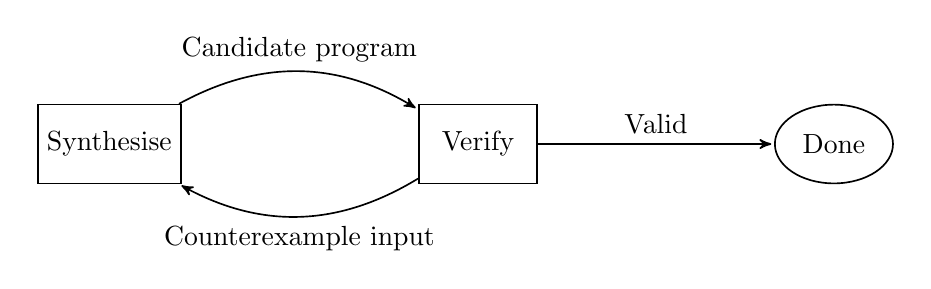
\begin{tikzpicture}[scale=0.5,->,>=stealth',shorten >=1pt,auto,
 semithick, initial text=]

  \matrix[nodes={draw, fill=none, scale=1, shape=rectangle, minimum height=1cm, minimum width=1.5cm},
          row sep=2cm, column sep=3cm] {
   \node (synth) {Synthesise};
   &
   \node (verif) {Verify}; %\\
   %\node[draw=none] {};
   &
   \node[ellipse] (done) {Done}; \\
  };

   \path
    (synth) edge [bend left] node {Candidate program} (verif)
    (verif) edge [bend left] node {Counterexample input} (synth)
    (verif) edge node {Valid} (done);
 \end{tikzpicture}
 
 \caption{Abstract synthesis refinement loop
 \label{fig:abstract-refinement}}
\end{figure*}



\begin{figure}
{\small
\begin{center}
\setlength{\tabcolsep}{16pt}
Integer arithmetic instructions:

\begin{tabular}{llll}
 \verb|add a b| & \verb|sub a b| & \verb|mul a b| & \verb|div a b| \\
 \verb|neg a| &   \verb|mod a b| & \verb|min a b| & \verb|max a b|
\end{tabular}

\medskip

Bitwise logical and shift instructions:

\begin{tabular}{lll}
 \verb|and  a b| & \verb|or   a b| & \verb|xor a b| \\
 \verb|lshr a b| & \verb|ashr a b| & \verb|not a|
\end{tabular}

\medskip

Unsigned and signed comparison instructions:

\begin{tabular}{lll}
 \verb|le  a b| & \verb|lt  a b| & \verb|sle  a b| \\
 \verb|slt a b| & \verb|eq  a b| & \verb|neq  a b|
\end{tabular}

Miscellaneous logical instructions:

\begin{tabular}{lll}
 \verb|implies a b| & \verb|ite a b c| & 
\end{tabular}

Floating point arithmetic:

\begin{tabular}{llll}
 \verb|fadd a b| & \verb|fsub a b| & \verb|fmul a b| & \verb|fdiv a b| 
\end{tabular}


\end{center}
}
 \caption{The language $\mathcal{L}$}
 \label{fig:l-language}
\end{figure}


\subsection{The Synthesis Algorithm}
As safety of a \newC program is efficiently 
%the quantifier free first-order fragment of the logic is efficiently 
decidable and a termination proof is expressible as a ground term of the \newC logic, we use
Counterexample Guided Inductive Synthesis (CEGIS)~\cite{lezama-thesis,sketch} to
check the validity of the synthesis formula. 
The core of the CEGIS algorithm is the refinement loop shown in Fig.~\ref{fig:abstract-refinement} and
detailed in Algorithm~\ref{fig:abstract-refinement-code}.  
The algorithm is divided into two
procedures: {\sc synth} (see Figure~\ref{fig:synth-dfd}) and {\sc verif}, which interact via
a finite set of test vectors {\sc inputs}, which is initialised to $\emptyset$.

The {\sc synth} procedure tries to find existential witnesses $(P, x_0)$ which satisfy the partial specification:
\[
 \exists P, x_0 . \forall x \in \text{\sc inputs} . \sigma(P, x_0, x)
\]

If {\sc synth} succeeds in finding a witness $(P, x_0)$, this witness is a candidate solution to the full
synthesis formula.  We pass this candidate solution to {\sc verif} which determines whether the candidate
does satisfy the specification on all inputs by checking satisfiability of the verification formula:
\[
 \exists x . \lnot \sigma(P, x_0, x)
\]

If this formula is unsatisfiable, the candidate solution is in fact a solution to the synthesis formula
and so the algorithm terminates.  Otherwise, the witness $x$ is an input on which the candidate solution fails
to meet the specification.  This witness $x$ is added to the {\sc inputs} set and the loop iterates again.

Concretely, {\sc synth} is implemented as shown in Figure~\ref{fig:synth-dfd}.  We start by taking the termination
specification and generating a C program which takes as input a candidate $(P, x_0)$ and asserts that the candidate
fails to meet the specification on at least on of the elements of {\sc inputs}.  So this program is unsafe iff there
is some candidate $(P, x_0)$ satisfying the specification for all the elements of {\sc inputs}.  Finding a new
candidate solution is therefore reduced to model checking this C program, which by construction is loop free.
The model checking is done using a combination of bounded model checking, explicit state enumeration and
genetic programming (GP).  The latter two techniques involve combining the previously generated C program,
along with code that searches for candidate solutions.  As well as efficiency, this has the side effect of
guaranteeing that we are verifying the exact semantics of the program under analysis as understood by a
compiler, rather than some ad-hoc abstraction of its semantics.  Finally, if any of the model checkers
finds a candidate solution it returns it.  The form of this candidate solution is yet another program,
this time written in the proof language $\mathcal{L}$.

Similarly, the {\sc verif} procedure is implemented by creating a C program that is unsafe iff
some input exists on which the candidate solution fails to meet the specification.  Again, symbolic
and explicit state model checking are used to decide the satisfiability of the verification formula.


%If the input set is finite, this procedure is guaranteed to terminate.



%% In some cases, it is faster to use an explicit-state model checker rather than a Bounded Model Checker.  
%% This is particularly true for the {\sc verif} component, 
%% where we have observed that incorrect programs tend
%% to be incorrect on a large fraction of the input space.  Counterexamples
%% are then very easy to find by explicit enumeration of a few inputs.
%% Since \newC is a fragment of C, we can generate an explicit-state
%% model checker using the same source files that we pass to {\sc cbmc}
%% and adding a small function to enumerate possible inputs.



%% ---  We begin with the program under analysis (the PUA).  From this we produce a specification (in second order logic)
%% encoding the termination of the PUA.  From the logical specification, we produce a program SYNTH.
%% SYNTH takes as input a proof and asserts that the proof is incorrect on at least one of the inputs being tracked so far.
%% Therefore, SYNTH is unsafe iff there is some proof that is correct for all of the tracked inputs.  Now we use testing
%% techniques to try to find a proof that causes SYNTH to crash.  The testing techniques we use are: model checking,
%% exhaustive search and genetic programming.  For the latter 2 techniques, we combine SYNTH with another program
%% (GP or EXPLICIT respectively) to create a program that searches for test vectors (proofs) that cause SYNTH
%% to crash.


%% In the {\sc synth} component, in order to find a candidate proof $P$ satisfying
%% $\sigma(i_1, P(i_1)) \land \ldots \land \sigma(i_N, P(i_N))$
%% for the tracked inputs $(i_1, \ldots, i_N)$, 
%% we attempt a safety proof.
%In order to determine the validity of the {\sc synth} formula, we can
%check the {\sc synth} program for safety.  


\begin{figure*}
\begin{center}
\tikzstyle{file}=[draw, text width=7.0em, text centered,
  minimum height=1.5em]
\tikzstyle{process} = [draw, minimum height=3em, circle]
\tikzstyle{line} = [draw, color=black, -latex']

\def\Divide#1#2{%
 \coordinate(a) at ($(#1.east) !.5! (#2.west)$);
 \coordinate(b) at (a |- 0,-3);
 \draw[dotted] (b) -- ++(0, 4.5);
}

\resizebox{\linewidth}{!}{
\begin{tikzpicture}[font=\sffamily]

\node [file] (pua) {input.c};

\path (pua.east)+(2,0) node [file] (spec) {\sc Termination Specification};
\path (spec.south)+(0.0, -1) node [file] (inputs) {\sc Tracked Inputs};
%% \path (synth.south)+(0.0, -0.5) node [file] (tests) {\sc tests.c};
%% \path (tests.south)+(0.0, -0.5) node [file] (interpreter) {\sc interpreter.c};
%% \path (interpreter.south)+(0.0, -0.5) node [file] (spec) {\sc spec.c};

%% \path (spec.east)+(2.0, -0.25) node [process] (merged) {merge};
\path (spec.east)+(2.0, -0.75) node [file] (file) {synth.c};

\path (file.east)+(2.0, 1.5) node [process] (cbmc) {\sc cbmc};
\path (file.east)+(2.0, 0.0) node [process] (gcc) {\sc Search};
\path (file.east)+(2.0, -1.5) node [process] (gp) {\sc GP};

\path (gcc.east)+(2.5, 0.0) node [file] (out) {Candidate Proof};

%\path [line] (spec) -- (merged);

\path [line] (pua) -- (spec);

\path [line] (spec) -- (file);
\path [line] (inputs) -- (file);

\path [line] (file) -- (cbmc);
\path [line] (file) -- (gcc);
\path [line] (file) -- (gp);


\path [line] (cbmc) -- (out);
\path [line] (gcc) -- (out);
\path [line] (gp) -- (out);

\Divide{pua}{spec}{puaspec}
%\Divide{spec}{file}{specfile}
\Divide{file}{gcc}{filegcc}
\Divide{gcc}{out}{gccout}

\draw (pua |- 0,-3) node [align=center] {Input program \\ (written in C)};

\coordinate (midspec) at ($(spec) !.5! (file)$);
\draw (midspec |- 0,-3) node [align=center] {Automatically generated specification \\ (written in C)};
%\draw (file |- 0,-3) node {Spec};
\draw (gcc |- 0,-3) node [align=center] {Model checker};
\draw (out |- 0,-3) node [align=center] {Proof \\ (written in $\mathcal{L}$)};

\end{tikzpicture}
}
\end{center}

\caption{Schematic diagram of {\sc synth}}
\label{fig:synth-dfd}
\end{figure*}


\subsection{Parameterising the Program Space}


In order to search the space of candidate programs, we parametrise
the language~$\mathcal{L}$ by program length, word width and number of constants,
inducing a lattice of progressively
more expressive languages.  We start by attempting to synthesise
a program at the lowest point on this lattice and increase the
parameters of~$\mathcal{L}$ until we reach a point at which
the synthesis succeeds.

As well as giving us an automatic search procedure, this parametrisation
greatly increases the efficiency of our system since languages
low down the lattice are very easy to decide safety for.  If a program
can be synthesised in a low-complexity language, the whole procedure
finishes much faster than if synthesis had been attempted in a
high-complexity language.


%% We introduce a novel parametrisation of the programming language
%% used to express our synthesised programs.
%% This parametrisation allows us to efficiently explore the program space
%% without relying on human guidance and also ensures that our programs
%% are of minimal length.

%% Our tool is the first we are aware of that is able to effectively
%% synthesise floating-point programs. We demonstrate this by
%% synthesising {\sc Fast2Sum} using Knuth's {\sc 2Sum}~\cite{taocp2} as
%% a specification.

%% ---Our exploration of the program space ensures that our programs are minimal in size.
%% --- We parametrise the space of programs in such a way that it can be explored automatically, rather than asking a human for hints.


%% We consider the following parameters:
%% \begin{itemize}
%% \item{Program Length: $l$}
%% The first parameter we introduce is program length, denoted by $l$.
%% At each iteration we synthesise programs of length exactly $l$.
%% We start with $l = 1$ and increment $l$ whenever we determine
%% that no program of length $l$ can satisfy the specification.  When we do
%% successfully synthesise a program, we are \emph{guaranteed that it
%% is of minimal length} since we have previously established that no
%% shorter program is correct.
%\item{Word Width: $w$}
%% An $\mathcal{L}$-program runs on a virtual machine (the $\mathcal{L}$-machine) that
%% has its own set of parameters.  The only relevant parameter is
%% the \emph{word width} of the $\mathcal{L}$-machine, that is, the number of bits
%% in each internal register and immediate constant.  This parameter is denoted by
%% $w$.  The size of the final SAT problem generated by {\sc cbmc} scales
%% polynomially with $w$, since each intermediate C variable corresponds
%% to $w$ propositional variables.


%\item{Number of Constants: $c$}
%% Instructions in $\mathcal{L}$ take either one or two operands.
%% Since any instruction whose operands are all constants can always be
%% eliminated (since its result is a constant), we know that a loop-free program
%% of minimal length will not contain any instructions with two constant
%% operands.  Therefore the number of constants that can appear in
%% a minimal program of length $l$ is at most $l$.  By minimising the number
%% of constants appearing in a program, we are able to use a particularly
%% efficient program encoding that speeds up the synthesis procedure
%% substantially.  The number of constants used in a program is the parameter $c$.

%\end{itemize}
%\subsubsection{Searching the Program Space}

The key to our automation approach is to come up with a sensible way in which to
adjust the $\mathcal{L}$-parameters in order to cover all possible programs.
After each round of {\sc synth}, we may need to adjust the parameters.  
%The
%logic for these adjustments is shown as a tree in Fig.~\ref{fig:paramsflow}.
Whenever {\sc synth} fails, we consider which parameter might have caused the
failure.  
%% There are two possibilities: either the program length $l$ was too small,
%% or the number of allowed constants $c$ was.  If $c < l$, we just increment $c$ and
%% try another round of synthesis, but allowing ourselves an extra program constant.
%% If $c = l$, there is no point in increasing $c$ any further.  This is because
%% no minimal $\mathcal{L}$-program has $c > l$, for if it did there would
%% have to be at least one instruction with two constant operands.  This
%% instruction could be removed (at the expense of adding its result as
%% a constant), contradicting the assumed minimality of the program.  So
%% if $c = l$, we set $c$ to 0 and increment $l$, before attempting
%% synthesis again.

%% If {\sc synth} succeeds but {\sc verif} fails, we have a candidate
%% program that is correct for some inputs but incorrect on at least
%% one input.  However, it may be the case that the candidate program
%% is correct for \emph{all} inputs when run on an $\mathcal{L}$-machine
%% with a small word size.  For example, we may have synthesised a
%% program which is correct for all 8-bit inputs, but incorrect for
%% some 32-bit input.  If this is the case (which we can determine
%% by running the candidate program through {\sc verif} using the smaller
%% word size), we may be able to produce a correct program for
%% the full $\mathcal{L}$-machine by using the constant extension rules
%% shown in Fig.~\ref{fig:generalize}.  If constant generalization
%% is able to find a correct program, we are done.  Otherwise,
%% we need to increase the word width of the $\mathcal{L}$-machine
%% we are currently synthesising for.


%% \section{Conclusion}

%% By expressing the program synthesis problem as a safety property for a
%% program interpreter, we have been able to harness the power of
%% state-of-the-art program analysis tools and reuse them in a new problem
%% domain.  We have implemented our algorithm as a freely downloadable tool
%% whose performance compares favourably to a recent program synthesiser. 
%% Finally, we have taken advantage of the expressiveness of our specification
%% language to make an initial step towards practical synthesis of
%% floating-point programs.




\section{Genetic Programming and Incremental Evolution}

We begin by observing that the asymptotic complexity of all of our synthesis
backends are equal, assuming $P \neq NP$.  This complexity is:

$$O(2^{K(f)}$$

Where $K(f)$ is the Kolmogorov complexity of $f$, which is $O(\log Y^X) = O(X)$
so the complexity is doubly exponential in the width of $X$.

\begin{definition}
 A \emph{fitness landscape} is the space of all programs along with their fitness.
\end{definition}

\begin{theorem}
 Fitness landscapes form a lattice.  Adding test vectors corresponds to abstraction refinement on this
 lattice, which is why incremental GP works well.
\end{theorem}

\begin{proof}
 Trivial.
\end{proof}


\begin{conjecture}
 A single fitness landscape isn't really very smooth (e.g. small changes in program representation
 don't correspond to small changes in fitness), so GP probably shouldn't work very well.
 
 But it does.
\end{conjecture}



\section{Experiments}

We proved termination for a bunch of programs, see Fig.~\ref{fig:linear} and Fig.~\ref{fig:nonlinear}.

\begin{figure*}
\centering
\begin{tabular}{|l|r|r||r|r|r|r|}
\hline
    & LOC & \shortstack{Rank function \\ size} & \textsc{T2} & \textsc{ARMC} & \textsc{Headshot} & \textsc{Headshot-Linear} \\
    \hline
    \hline
 P1 & 10 & 3 & 100s & 70s & 0.1s & \bf{0.01s} \\
 P2 & 10 & 3 & 100s & 70s & 0.1s & \bf{0.01s} \\
 P3 & 10 & 3 & 100s & 70s & 0.1s & \bf{0.01s} \\
 \hline
\end{tabular}
\caption{Termination for linear programs with disjunctive, linear ranking functions\label{fig:linear}}
\end{figure*}

\begin{figure*}
\centering
\begin{tabular}{|l|r|c|c|c|c|r|r|r|}
\hline
    & LOC & \shortstack{Linear \\ program?} & \shortstack{Linear ranking \\ function?}  & Conditional? & Float? & Dimension & \shortstack{Ranking \\ program size} & Time (s)\\
    \hline
    \hline
 P1 & 10 & \xmark & \xmark & \xmark & \xmark & 3 & 1 & 0.01 \\
 P2 & 10 & \xmark & \xmark & \xmark & \xmark & 3 & 1 & 0.01 \\
 P3 & 10 & \xmark & \xmark & \xmark & \xmark & 3 & 1 & 0.01 \\
 \hline
\end{tabular}

\caption{\textsc{Headshot} termination for nonlinear programs with nonlinear ranking functions\label{fig:nonlinear}}
 \end{figure*}


\bibliographystyle{abbrvnat}
\bibliography{synth}{}

\end{document}
